\documentclass[aspectratio=169,11pt]{beamer}
\usepackage{fontspec}
\setsansfont{Noto Sans}
\setmainfont{Noto Sans}
\usepackage{tikz}
\usetikzlibrary{arrows.meta,positioning,calc}
\usepackage{graphicx}

\setbeamertemplate{navigation symbols}{}
\setbeamertemplate{headline}{}
\setbeamertemplate{frametitle}{\vspace{0.35cm}\insertframetitle\par\vspace{0.10cm}}
\setbeamertemplate{footline}{\hfill\usebeamerfont{page number in head/foot}\insertframenumber\hspace{0.8cm}\vspace{0.25cm}}
\setbeamercolor{normal text}{fg=black,bg=white}
\setbeamercolor{frametitle}{fg=black,bg=white}
\setbeamercolor{structure}{fg=black}
\setbeamercolor{page number in head/foot}{fg=black!55}
\setbeamerfont{normal text}{size=\large}
\setbeamerfont{frametitle}{size=\LARGE,series=\bfseries}
\setbeamerfont{page number in head/foot}{size=\small}
\setbeamersize{text margin left=0.8cm,text margin right=0.8cm}
\setlength{\parskip}{0.55em}
\hypersetup{pdftitle={COLMIX — Máy pha màu theo khối lượng},pdfauthor={},pdfsubject={Mô hình thử nghiệm IoT},pdfkeywords={COLMIX, IoT, định lượng}}

\newcommand{\simcaption}{\vspace{0.06cm}{\fontsize{9}{12}\selectfont Minh họa mô phỏng, bộ điều khiển Rust chạy trên máy tính\par}}
\newcommand{\smalllabel}[1]{{\fontsize{11}{14}\selectfont #1}}

\begin{document}

\begin{frame}{COLMIX}
\vspace{0.12cm}
{\LARGE Máy pha màu theo khối lượng\par}
{\large Mô hình thử nghiệm IoT\par}
\vspace{0.45cm}
Hướng đến pha màu theo công thức, kết hợp cân định lượng, khuấy trộn và giám sát qua giao diện web
\vspace{0.55cm}
\begin{center}
\begin{tikzpicture}[node distance=0.7cm, every node/.style={font=\normalsize}, stage/.style={draw=black!60, minimum width=3.5cm, minimum height=0.85cm}, >={Stealth[length=2mm]}]
\node[stage] (recipe) {Công thức};
\node[stage,right=of recipe] (dose) {Định lượng};
\node[stage,right=of dose] (mix) {Khuấy trộn};
\draw[->] (recipe) -- (dose);
\draw[->] (dose) -- (mix);
\end{tikzpicture}
\end{center}
\end{frame}

\begin{frame}{Nhu cầu sử dụng}
\vspace{0.3cm}
Mục tiêu là giúp tái sử dụng tỉ lệ pha, theo dõi lượng cấp và quan sát trạng thái mẻ
\vspace{0.8cm}
\begin{columns}[T,onlytextwidth]
\begin{column}{0.30\textwidth}\textbf{Lớp thực hành}\end{column}
\begin{column}{0.30\textwidth}\textbf{Xưởng thủ công}\end{column}
\begin{column}{0.30\textwidth}\textbf{Mẻ màu nhỏ}\end{column}
\end{columns}
\vspace{0.5cm}
Hướng đến thao tác gọn và công thức rõ ràng
\end{frame}

\begin{frame}{Mô hình thử nghiệm}
\vspace{-0.05cm}
\begin{center}
\begin{tikzpicture}[x=1cm,y=1cm, font=\fontsize{10}{13}\selectfont, >={Stealth[length=1.8mm]}, tank/.style={draw=black!70,minimum width=2.65cm,minimum height=1.05cm,align=center}, pump/.style={draw=black!70,circle,minimum size=0.55cm,inner sep=1pt}]
\node[tank] (a) at (-4,2.2) {Xanh lá 066\\Phao · khuấy};
\node[tank] (b) at (0,2.2) {Màu da 046\\Phao · khuấy};
\node[tank] (c) at (4,2.2) {Xanh dương 035\\Phao · khuấy};
\node[pump] (pa) at (-4,0.95) {P1};
\node[pump] (pb) at (0,0.95) {P2};
\node[pump] (pc) at (4,0.95) {P3};
\node[draw=black!70,minimum width=3.5cm,minimum height=0.85cm,align=center] (cup) at (0,-0.25) {Cốc nhận · khuấy};
\node[align=center] (scale) at (0,-1.2) {Loadcell 1 kg · HX711};
\draw[->] (a) -- (pa);\draw[->] (b) -- (pb);\draw[->] (c) -- (pc);
\draw[->] (pa.south) |- (cup.west);\draw[->] (pb) -- (cup);\draw[->] (pc.south) |- (cup.east);
\draw (cup.south) -- (scale.north);
\end{tikzpicture}
\end{center}
\vspace{0.05cm}
Nguồn 12 V qua các bộ hạ áp, cấp cho khối điều khiển và động cơ
\end{frame}

\begin{frame}{Kiến trúc đề xuất}
\vspace{0.35cm}
\begin{center}
\begin{tikzpicture}[font=\fontsize{12}{15}\selectfont, >={Stealth[length=1.8mm]}, box/.style={draw=black!70,minimum width=2.7cm,minimum height=1.15cm,align=center}]
\node[box] (esp) at (0,0) {ESP32\\Rust};
\node[box] (mqtt) at (3.7,0) {Bộ chuyển tiếp\\MQTT};
\node[box] (go) at (7.4,0) {Máy chủ\\Go};
\node[box] (web) at (11.1,0) {Giao diện\\web};
\draw[<->] (esp) -- node[above,font=\fontsize{9}{11}\selectfont] {Wi-Fi} (mqtt);
\draw[<->] (mqtt) -- (go);
\draw[<->] (go) -- node[above,font=\fontsize{9}{11}\selectfont] {WebSocket} (web);
\node[font=\fontsize{10}{13}\selectfont] at (5.55,-1.15) {Lệnh điều khiển $\longleftrightarrow$ Trạng thái và dữ liệu cân};
\end{tikzpicture}
\end{center}
\vspace{0.5cm}
Khối điều khiển hướng đến vận hành mẻ tại thiết bị, máy chủ chuyển lệnh và cập nhật giao diện
\end{frame}

\begin{frame}{Thiết lập công thức}
\begin{columns}[c,onlytextwidth]
\begin{column}{0.52\textwidth}
Mẻ minh họa 100 g, tỉ lệ khối lượng xanh lá, màu da, xanh dương là 50/30/20
\vspace{0.5cm}
{\Large $50 + 30 + 20 = 100$ g\par}
\end{column}
\begin{column}{0.40\textwidth}
\centering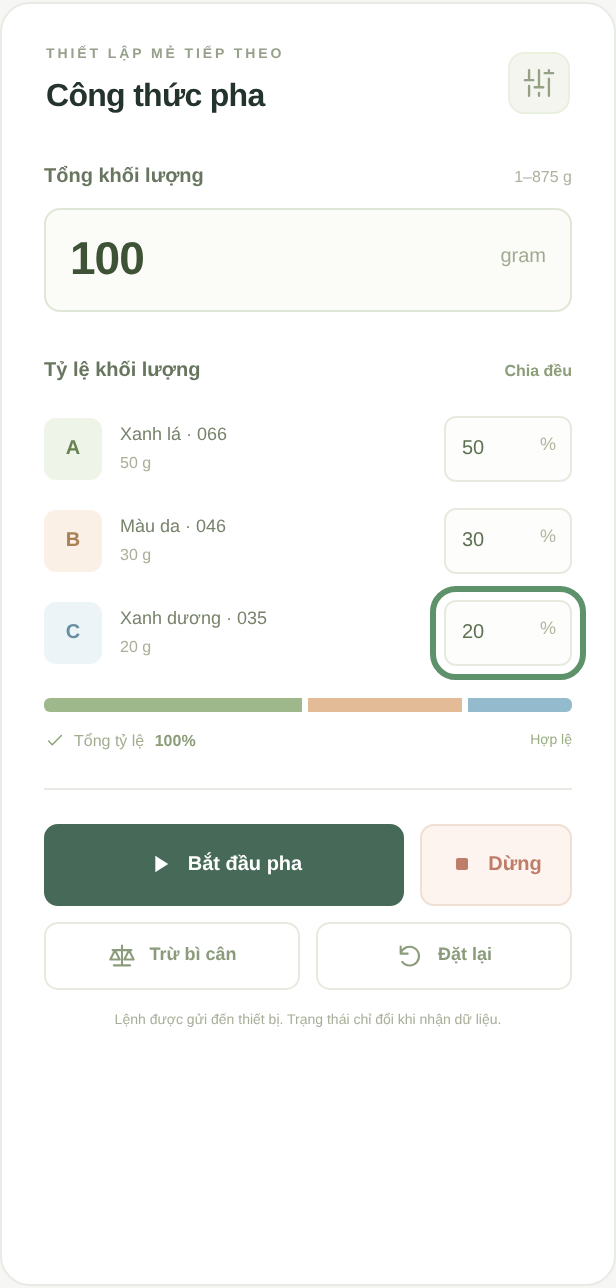
\includegraphics[height=5.55cm]{assets/01-setup.png}
\end{column}
\end{columns}
\simcaption
\end{frame}

\begin{frame}{Định lượng theo cân}
\begin{columns}[c,onlytextwidth]
\begin{column}{0.27\textwidth}
Mục tiêu là cấp lần lượt ba màu, cân phản hồi lượng đã cấp theo công thức
\vspace{0.3cm}

\includegraphics[width=\linewidth]{assets/02-dosing-state.png}
\end{column}
\begin{column}{0.70\textwidth}
\centering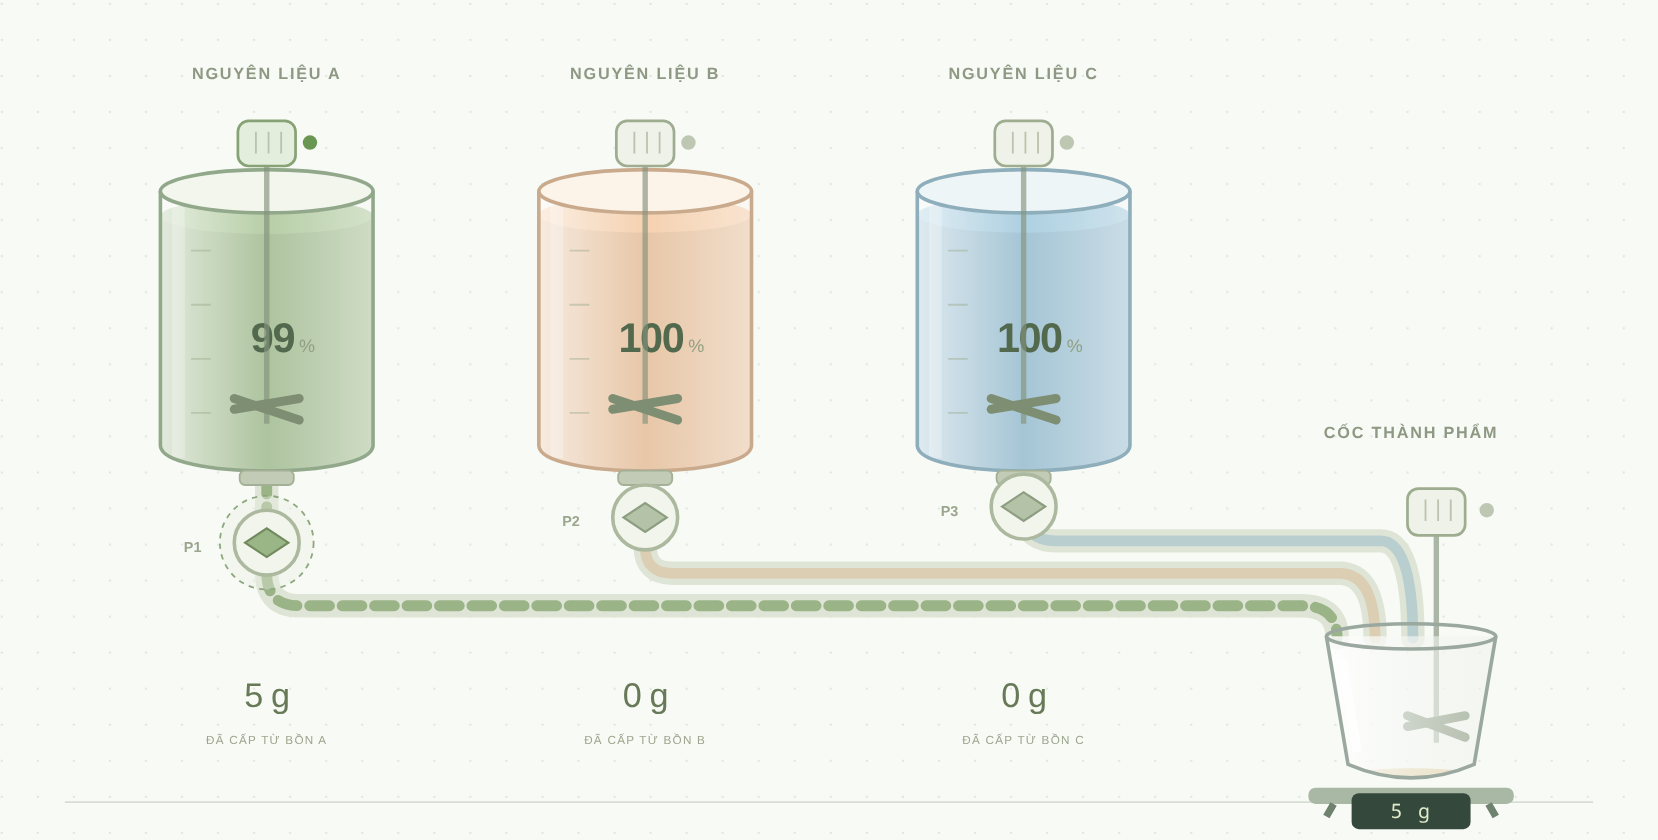
\includegraphics[width=\linewidth]{assets/02-dosing.png}
\end{column}
\end{columns}
\simcaption
\end{frame}

\begin{frame}{Khuấy trộn tại cốc nhận}
\begin{columns}[c,onlytextwidth]
\begin{column}{0.63\textwidth}
Hướng đến khuấy hỗn hợp sau định lượng, theo dõi trạng thái bộ khuấy và khối lượng trên giao diện
\vspace{0.25cm}
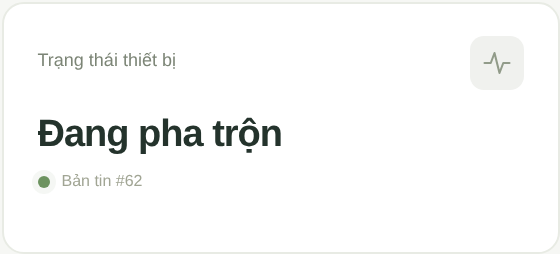
\includegraphics[width=4.2cm]{assets/03-mixing-state.png}
\end{column}
\begin{column}{0.30\textwidth}
\centering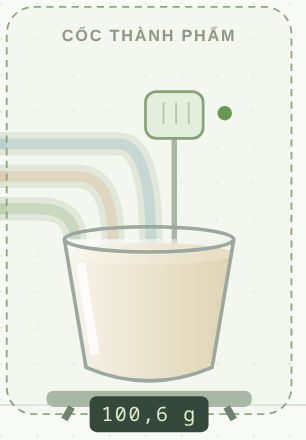
\includegraphics[height=5.25cm]{assets/03-mixing.png}
\end{column}
\end{columns}
\simcaption
\end{frame}

\begin{frame}{Theo dõi mẻ pha}
Mô hình thử nghiệm hiển thị diễn biến khối lượng, trạng thái hoàn tất và sự kiện của mẻ
\vspace{0.05cm}
\begin{columns}[T,onlytextwidth]
\begin{column}{0.66\textwidth}
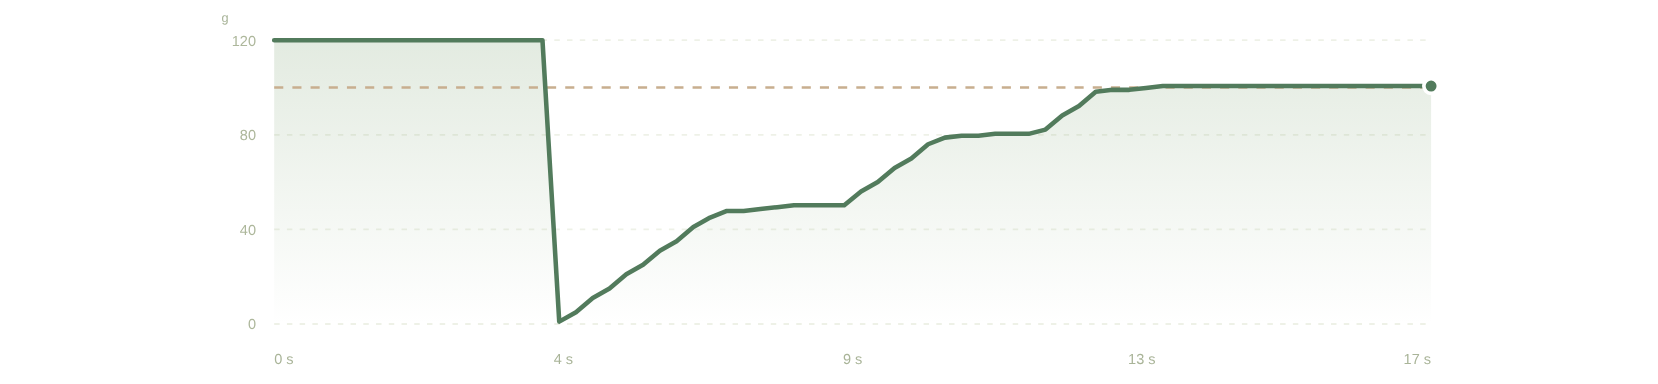
\includegraphics[width=\linewidth]{assets/04-complete-chart.png}
\vspace{0.05cm}

\includegraphics[width=\linewidth]{assets/04-complete-log.png}
\end{column}
\begin{column}{0.30\textwidth}
\vspace{0.25cm}
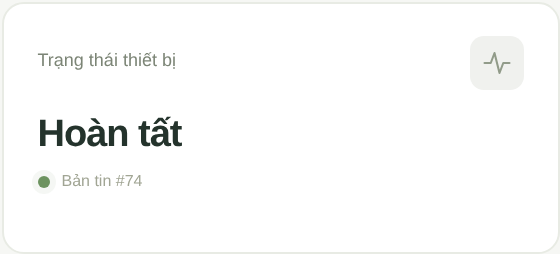
\includegraphics[width=\linewidth]{assets/04-complete-state.png}
\end{column}
\end{columns}
\simcaption
\end{frame}

\begin{frame}{Giá trị hướng đến}
\vspace{0.5cm}
Mục tiêu là công thức dễ lặp lại, định lượng tự động và giám sát thuận tiện
\vspace{0.9cm}
Nếu phù hợp với vật liệu, mô hình có thể hỗ trợ pha màu mẻ nhỏ
\end{frame}

\end{document}
